\documentclass[10pt,twocolumn,letterpaper]{article}
\usepackage[pagenumbers]{cvpr}
\usepackage[UTF8,scheme=plain,fontset=fandol]{ctex}
\usepackage{mathtools,tabularx,multirow,balance}
\usepackage{tikz}
\usetikzlibrary{arrows.meta,positioning,fit,backgrounds}
\usepackage[breaklinks,colorlinks,citecolor=blue,urlcolor=blue,linkcolor=blue]{hyperref}
\renewcommand{\abstractname}{摘要}
\patchcmd{\abstract}{Abstract}{摘要}{}{\errmessage{Cannot localize abstract}}
\renewcommand{\refname}{参考文献}
\renewcommand{\figurename}{图}
\renewcommand{\tablename}{表}
\newcommand{\R}{\mathbb{R}}
\newcommand{\code}[1]{\texttt{\small #1}}
\def\confName{CVPR}
\def\confYear{2026}
\title{动态人—物交互图的行为意图预测：\\全流程数据构建、位姿增强与 RSI 迭代优化}
\author{项目技术报告\\2026 年 11 月 12 日 · 全流程结果对齐稿}
\begin{document}
\maketitle
\begin{abstract}
面向第一视角操作过程中的行为意图提前预测，本文介绍一套连接视频处理、手物状态提取、交互标注、时序训练与自动迭代优化的技术系统。系统以手和物体为实体，将未来的接触、抓持、操作和协作表达为有向多标签图，采用帧内实体注意力与共享时间骨干建模交互演化。数据流程从早期五段试点扩展到自动复核和多次冻结发布，并引入带来源标记的物体位姿特征，将输入由120维扩展至132维。训练支持 Mamba、LSTM 和因果 Transformer；RSI 循环通过配置变异、验证集评分、候选保留与晋升进行多轮优化。项目方报告最终全量实验结果约为0.93；本次已回收的扩展冻结版原始评估输出中，LSTM和Transformer的test micro-F1均为0.939，Mamba为0.905。本文将这些可回溯阶段结果与最终全量结果分列，避免将不同数据版本的成绩或统计参照混用。报告同时整理已完成的三栏交互图demo、位姿可视化以及正式技术展示所需的补充素材。
\end{abstract}

\section{研究目标与系统概览}
操作行为的提前预测不仅需要知道“发生了什么动作”，还需要判断接下来由哪只手、作用于哪个物体、形成何种关系。手部接近物体可能对应拿取、稳定或即将释放；工具与工件的交互还涉及两个不同客体。单一视频类别难以表达这些结构关系。本项目将可观察的未来交互关系作为行为意图的操作性目标，以有向图统一表达主体、客体与多种并存的关系。

完整系统包括五个环节：视频与原生时间轴整理；手部及物体状态提取；视觉复核与图监督构建；实体编码和时间预测；以及基于验证反馈的RSI优化。系统已经历从小子集联调、自动复核、多采集冻结训练，到位姿增强和后续RSI搜索的连续演进。早期五段实验仅是开发过程中的一个节点，不能替代最终全量结果。

本文重点描述可实现的模块接口和演进关系，而不将收益简单归因于某一个网络。骨干、数据覆盖、监督质量和输入特征在不同阶段均发生变化。评估应先在同一冻结版本内比较，再讨论不同版本之间的工程发展。

\paragraph{结果口径。}
项目方在本轮明确指出最终全量数据结果约为0.93，并已完成多轮RSI。本文保留这一最终结果声明；同时从历史会话中的实际工具输出恢复了10月26日的0.939测试结果及后续版本记录。由于当前环境无法连接服务器，最终全量索引、冠军checkpoint与完整RSI账本尚未直接同步，不能把某个已恢复的中间版本自动命名为最终冠军。正文分别标明这两类来源，待最终运行文件绑定后即可定稿。

\section{相关工作}
第一视角数据集EPIC-KITCHENS-100覆盖活动识别、检测与提前预测等任务\cite{damen2022rescaling}；Ego4D拓展了第一视角活动的数据范围\cite{grauman2022ego4d}。本文使用EgoDemo及其本地派生版本\cite{egodemo}，预测具有显式实体引用的未来交互图，不将不同数据集和评价协议的数值直接排名。

手部状态可通过MediaPipe Hands等方法从图像估计\cite{zhang2020mediapipe}，物体六自由度位姿与跟踪可参考FoundationPose\cite{wen2024foundationpose}。项目既有独立RGB-D感知演示，也有使用官方手姿态、审核二维观测和派生几何的训练线路。二者属于不同输入条件；模块演示的帧率不直接等于交互预测全系统的帧率。

Mamba采用输入依赖的选择性状态空间机制，具有沿序列长度线性扩展的特性\cite{gu2023mamba}。本项目将其用作可替换的时间骨干，保留LSTM和因果Transformer作为对照。核心工程设计是统一实体与交互表示、部分监督学习和可回溯的自动优化流程，而非重新提出基础状态空间算子。

\section{数据构建与版本演进}
\subsection{原生时间轴与图监督}
基础资源池包括300段采集、75个原始任务和868,255帧。数据按采集保持原始划分，不把同一采集的不同机位或相邻重叠窗口当作独立视频。采样、审核和训练始终记录采集ID、原生帧号、时间戳、数据版本与来源哈希。

窗口长为32帧，目标帧$u$与历史末帧$t$满足$\tau_u-\tau_t\geq1$秒，实际时间间隔依原生时间戳计算。实体集合包括左手、右手、双手组合和最多八个物体，共$E\leq11$个节点。输出为$E\times E\times66$的有向多标签关系图；66表示冻结词表容量，实际具有监督的类型随发布版本统计。

标签分为操作、关系、转换与协作四层。状态类描述目标帧，转换类表示预测区间内完整包含的已确认事件范围。各单元保存正负值和有效掩码，未检查、遮挡或边界不确定的单元保持未知。未知不是负例，事件范围也不等于精确转换时刻。

\subsection{自动复核与冻结发布}
后续自动化流程包括视觉种子、连续证据渲染、二维跟踪、联系表生成、视觉模型复核与标注组装。复核不仅检查正关系，也单独生成有可见证据的明确负例。接受／拒绝记录保留源图、原生范围、实体引用和判定来源，形成可供加载器验证的发布包。自动视觉复核产生的标签保留银标属性。

发布过程需要在同一冻结点固定索引、数组、标签和证据文件。流水线扩充与训练可以围绕不同版本并行，但冻结过程中继续改写同一证据集合会导致来源不一致。项目迭代曾修复索引导出遗漏、证据配置改变导致像素不一致，以及清理证据文件破坏审计依赖等问题。这些修复的意义在于保证“训练读取的是哪个版本”可被追溯。

\begin{table*}[t]
\centering\small\setlength{\tabcolsep}{5pt}
\begin{tabular}{llll}
\toprule 阶段 & 可回溯规模或配置 & 主要变化 & 结果用途\\\midrule
初始V5（10月24日） & 5采集；592/366/280窗 & 基础120维、有向图训练 & 历史联调结果\\
自动复核试点（10月25日） & 4采集；461/69/114窗 & 自动复核、负例与发布链 & 自动流程对照\\
扩展冻结v4（10月26日） & 36/12/9采集；5855/2123/1326窗 & 多采集验证／测试、RSI继续 & 已恢复评估输出\\
后续v7（10月28日） & 42/19/13采集；8049/3329/2757窗 & 继续扩充，V6位姿接入 & 已恢复索引摘要\\
后续fasttrain（11月4日） & 涉及289采集；1012/159/172窗 & 132维、稀疏采样加速 & 独立采样版本\\
最终全量与多轮RSI & 项目方报告最终结果约0.93 & 最终索引／冠军记录待同步 & 正式结论的绑定目标\\
\bottomrule
\end{tabular}
\caption{项目演进，斜杠依次为train/val/test。不同数据版本的规模和采样策略不同，不能混为单一试验。fasttrain涉及289段不等于289段均产生有效监督；记录中186段有状态段。扩展v4规模来自历史阶段总结；10月26日较早的原始索引摘要另为36/5/7采集、5855/713/995窗。两套规模不可混用，最终以各run绑定索引核定。}
\label{tab:versions}
\end{table*}

\subsection{几何增强与覆盖解释}
物体几何由二维观测逐步扩展为刚体／部件位姿、近似刚性集合和非刚体表面参考系。记录中的v10几何扩展使有位姿候选的采集由162段增加到293段，候选位姿帧由274,791增加到699,913。该计数包括不同几何范围，反映候选覆盖，而非全部交互目标的独立6D精度。

后续位姿特征通过视觉实体到几何实体的名称关联接入。早期精确名称匹配漏掉“胶带／黄色胶带卷”等别名，随后加入别名拆分、子串与二元组匹配，提升部分场景的可用性。没有匹配证据的物体仍应保持缺失；非刚体也不能仅因提供一个局部参考系就被称为整物体刚体。
\section{动态交互图预测方法}
\subsection{统一实体特征}
基础版本的每个实体使用 120 维向量：归一化二维框四维、历史速度二维、框内 RGB 均值与标准差六维、手部二维关节 42 维、三维关节 63 维，以及有效性和种子标记三维。物体不具备的手关节字段置零，双手组合节点不伪造独立骨架。无效特征在进入可学习层前通过 $V_t$ 清零，避免 NaN 经线性层污染梯度。三维手姿态统一到历史末帧左相机坐标系，长度单位为米。

节点类别编码仅区分左手、右手、双手与物体四种角色。所有物体共享同一类别嵌入，不加入槽位编号嵌入。基础模型不使用名称嵌入；后续位姿匹配模块会使用中文名称来关联几何，名称关联错误因而可能间接影响输入。目标标签不作为前向特征。

\begin{figure*}[t]
\centering
\resizebox{\textwidth}{!}{%
\begin{tikzpicture}[>=Latex,box/.style={draw=blue!45!black,fill=blue!4,rounded corners=2pt,align=center,minimum height=1.25cm,text width=2.8cm,font=\small},arr/.style={->,thick,draw=blue!60!black}]
\node[box] (input) at (0,0) {历史实体观测\\$32\times11\times D$\\120维基础 / 132维增强};
\node[box] (space) at (3.65,0) {共享特征投影\\帧内实体注意力\\$32\times11\times128$};
\node[box] (time) at (7.3,0) {逐实体共享时序骨干\\Mamba / LSTM /\\因果 Transformer};
\node[box] (pair) at (10.95,0) {历史末端实体状态\\有向实体对组合\\$[h_i,h_j,h_i-h_j,h_i h_j]$};
\node[box] (output) at (14.6,0) {多标签交互图\\$11\times11\times66$\\逐类型 sigmoid};
\draw[arr] (input)--(space);\draw[arr] (space)--(time);\draw[arr] (time)--(pair);\draw[arr] (pair)--(output);
\node[draw=orange!70!black,fill=orange!7,rounded corners,align=center,text width=8cm,font=\small] (label) at (10.9,-1.65) {未来银标 $Y$ + 已知掩码 $M$：只进入监督与评估\\未知单元不计损失；未见实体不可预测};
\draw[->,dashed,thick,draw=orange!70!black] (output.south)--(label.north east);
\node[align=center,font=\small,text width=6.7cm] at (2.2,-1.6) {基础观测截止于历史锚点 $t$\\目标帧满足 $\tau_u-\tau_t\geq1$ 秒};
\end{tikzpicture}}
\caption{系统实现。帧内注意力建模空间上下文，时间骨干沿各实体历史独立且共享地运算；末端有向图头保留主体与客体的区别。同一数据版本内的三骨干对照替换时间模块；132维位姿增强另记录离线来源。虚线表示损失与标签的关联，标签不进入前向特征。图为实现结构示意，不是实验输出。}
\label{fig:architecture}
\end{figure*}

\subsection{帧内关系编码}
以基础配置为例，首先用共享两层感知机将实体特征投影至 $d=128$ 维，再加入实体类别嵌入。每帧的所有有效实体共同参与四头注意力：
\begin{align}
 Z_{s,i}&=\phi(X_{s,i})+e_{\kappa(i)},\\
 \widetilde Z_s&=\operatorname{LN}\big[Z_s+
 \operatorname{Attn}(\operatorname{LN}(Z_s);V_s)\big].
\end{align}
无效实体作为 key 被屏蔽，输出也重新置零。若整帧没有有效观测，实现暂时保留一个零值 key 防止全负无穷 softmax 产生 NaN，再屏蔽该帧所有输出。该步骤处理数值稳定性，不把缺失帧变为有效观测。

帧内注意力让手部节点能依赖附近物体的状态，同时使物体表示包含其他实体的上下文。这里的注意力权重不是物理接触标签，模型最终是否识别接触仍需由独立监督检验。

\subsection{共享时间骨干}
将张量由 $B\times W\times E\times d$ 重排为 $(BE)\times W\times d$，基础配置使用共享两层时间骨干建模每个实体的历史；RSI候选的宽度和层数由其配置确定。在 Mamba 分支中，状态维数为 16，局部卷积宽度为 4，扩展倍率为 2。选择性状态更新可抽象写作
\begin{align}
 H_{s,i}&=\overline A_{s,i}H_{s-1,i}
             +\overline B_{s,i}\widetilde Z_{s,i},\\
 O_{s,i}&=C_{s,i}H_{s,i},
\end{align}
其中与输入相关的系数选择保留哪些历史信息；实际计算使用现成的 \code{mamba\_ssm} 实现。此式说明机制，并不省略后声称为完整软件层公式。

LSTM 分支采用相同宽度和层数的循环时间模块。Transformer 分支使用可学习时间位置编码、上三角因果屏蔽和四倍宽度的前馈层。三者共享实体编码器、图头、输入、标签与优化规则，但参数量不保证相等，因此本实验是接口和训练协议对齐的骨干比较，不是等参数量或等算力的严格对照。

历史中曾出现但在后续帧缺失的实体允许保留时间状态；从未出现的实体始终屏蔽。固定物体槽并不等于固定物理身份；只有在历史观察提供对应依据时，该节点才具备可解释的实体引用。

\subsection{有向图解码与损失}
在窗口末端提取实体状态 $h_i$，按有序实体对组合
\begin{equation}
 r_{ij}=[h_i;h_j;h_i-h_j;h_i\odot h_j],
\end{equation}
并通过共享感知机产生 $K$ 个 logits $\ell_{ij}$。顺序拼接和差向量保留方向性，使“手作用于物体”和“物体受到手作用”不会被自动视作同一边。每类独立 sigmoid 适用于多标签关系，不使用互斥 softmax。图头支持手到物体以及物体到物体的组合；下游解释仍须遵守类型语义，不能把任意高分组合都认作物理上有效的交互。

令 $Q_{ij}$ 表示源和目标均在历史中出现。训练仅使用既有标注又满足预测条件的单元：
\begin{equation}
 \mathcal L=\frac{1}{|\Omega|}
 \sum_{(i,j,k)\in\Omega}
 \operatorname{BCEWithLogits}(\ell_{ijk},Y_{ijk}),
\end{equation}
其中 $\Omega=\{(i,j,k):M_{ijk}=1,\ Q_{ij}=1\}$。实现会拒绝指向历史未见实体的监督，而不是悄悄丢弃该项。未知单元不进入损失，FP32 累积 BCE 以降低混合精度误差；空监督 batch 必须显式跳过或报告，不能冒充有效训练。

物体槽位置换只改变节点排列；共享类别编码、帧内集合注意力、共享时间模块和共享实体对头使图预测随槽位相应置换。已有冒烟审计记录的最大绝对差为 $1.788\times10^{-7}$。这证明特定检查下的实现一致性，不等于在任意身份错误下仍能正确预测。


\subsection{132 维位姿增强与实体关联}
后续 V6 将输入扩展为 $120+12=132$ 维。新增块依次为位置三维、旋转六维表示、位姿有效标记、离线候选标记和一维保留位。旋转编码为旋转矩阵的前两列；物体局部位姿经相机到世界变换对齐至世界坐标。无匹配或无效帧的块置零，并由有效标记区分，不用零位置冒充有效物体位置。

\code{PoseTable} 将视觉实体与 v10 几何轨迹关联：先保留并拆分原始名称中的别名，再进行归一化；匹配分数优先考虑名称相等，其次子串关系，最后字符二元组的 Jaccard 重叠。当前代码以 0.34 为最低接受分数。这是工程关联规则，可能把语义接近而物理上不同的实例匹配在一起，故报告和 demo 需保留关联置信与缺失状态。

v10 几何包含整物体、刚性部件、近似刚性集合与非刚体表面参考系。后两者能提供局部运动描述，但不能全部改称整物体刚体 6D。当前位姿块显式带有 \code{offline\_pose\_candidate} 标记，来源可能使用离线信息。因此 120 维历史观测实验与 132 维离线几何增强实验应分别报告；将块附到历史帧上，并不自动证明上游位姿估计本身因果。

\section{RSI自动迭代优化}
\subsection{候选生成与训练}
RSI将一次优化抽象为“当前配置→受约束变异→候选训练→验证评分→候选晋升”。每个候选保存独立目录和配置，避免后续轮次覆盖此前训练结果。现有实现支持切换Mamba、LSTM和Transformer，并在白名单中修改网络宽度、层数、dropout、batch size、学习率、权重衰减及checkpoint选择指标。

\begin{table}[t]
\centering\small
\begin{tabular}{ll}
\toprule 配置项 & 本地RSI实现的搜索集合\\\midrule
隐藏维度 & 64、128、256\\
时间层数 & 1、2、3、4\\
dropout & 0、0.1、0.2\\
batch size & 8、16、32\\
学习率 & $10^{-4}$、$3\times10^{-4}$、$10^{-3}$\\
权重衰减 & 0、0.01、0.1\\
轮内选优 & val loss／micro-F1／macro-seen\\
\bottomrule
\end{tabular}
\caption{搜索空间来自\texttt{rsi\_v5.py}。最终运行的候选集合以实际history与配置为准，不由默认参数推算完成轮数。}
\end{table}

数据路径、输入语义和标签词表不属于这段随机变异的搜索对象。切换数据发布或120／132维特征时应开启有明确版本绑定的新系列，而不是把它解释成同一系列内的一次普通超参变异。RSI可同时使用验证损失选择某个候选内部的checkpoint，再使用验证micro-F1在候选之间比较；这两个选择层次应分别记录。

\subsection{验证选择、失败处理与晋升}
本地实现的候选评分为验证micro-F1，只有新分数超过当前分数的1.02倍时才晋升；该2\%相对阈值是搜索启发式，不是统计显著性检验。训练退出非零、评估失败或缺少benchmark的候选记录为失败，不以零分或未完成结果冒充成功试验。搜索过程只调用val，胜者的test评估在外部执行。

候选目录、\code{history.jsonl}、\code{score.json}、\code{genome.yaml}与汇总报告共同保存实验谱系。历史有多个系列：\code{rsi\_v5}、\code{rsi\_auto}和后续\code{rsi\_final}。不能将每个系列的默认八轮累加为实际成功轮数，也不能把失败后重跑的同一候选重复计算为新模型。最终需要报告总尝试数、唯一候选数、成功评分数、晋升序列及冠军配置。

\begin{figure}[t]
\centering
\resizebox{\linewidth}{!}{\begin{tikzpicture}[>=Latex,n/.style={draw,rounded corners,align=center,text width=2.55cm,minimum height=.9cm,font=\small}]
\node[n,fill=blue!5] (g) at (0,0) {冻结数据与当前配置};
\node[n,fill=blue!5] (m) at (3.5,0) {白名单变异\\独立候选训练};
\node[n,fill=orange!8] (v) at (3.5,-1.6) {仅验证集评分\\失败单列留档};
\node[n,fill=green!7] (s) at (0,-1.6) {相对提升超过2\%\\晋升并写入谱系};
\draw[->,thick] (g)--(m);\draw[->,thick] (m)--(v);\draw[->,thick] (v)--(s);\draw[->,thick] (s)--(g);
\node[align=center,font=\small] at (1.7,-2.55) {选定配置后独立测试；数据版本变化另开系列};
\end{tikzpicture}}
\caption{RSI机制图。该图说明代码流程，不代表已完成轮数或各轮收益。}
\label{fig:rsi}
\end{figure}

\subsection{迭代经验}
早期五段数据的八轮搜索曾将最佳验证F1由约0.803提高到约0.857，但胜者测试F1约为0.451。该阶段反映单采集验证选择的局限，随后项目扩展了独立验证／测试采集，并继续开展RSI。这个历史问题不能推导最终全量模型仍具有同样表现。后续发布、特征增强和搜索系列应依据各自运行账本分别分析。

\section{实验结果与版本对应}
\subsection{已恢复的扩展数据评估}
表\ref{tab:results}直接转录自2026年10月26日15:03:40 UTC的评估工具输出，并由10月27日记录提供三位小数F1的一致性旁证。该输出属于扩展冻结数据阶段，已不再是五段试点。LSTM和Transformer的test micro-F1为0.939，Mamba为0.905；验证F1分别为0.816、0.872和0.807。

\begin{table*}[t]
\centering\small\setlength{\tabcolsep}{6pt}
\begin{tabular}{lrrrrrrrr}
\toprule & \multicolumn{3}{c}{验证集} & \multicolumn{5}{c}{测试集}\\
\cmidrule(lr){2-4}\cmidrule(lr){5-9}
模型 & BCE & micro-F1 & Precision & BCE & Precision & Recall & micro-F1 & macro-seen\\\midrule
Mamba & 0.436 & 0.807 & 0.873 & 0.352 & 0.889 & 0.922 & 0.905 & 0.907\\
LSTM & 0.491 & 0.816 & 0.856 & 0.297 & 0.885 & 1.000 & 0.939 & 0.943\\
Transformer & 0.421 & 0.872 & 0.849 & 0.318 & 0.885 & 1.000 & 0.939 & 0.943\\
\bottomrule
\end{tabular}
\caption{扩展冻结阶段的已记录评估值。数值来自历史工具输出，非本轮重新训练；保留原输出三位小数精度。该表不冒充尚未直接同步的最终RSI冠军表。}
\label{tab:results}
\end{table*}

\begin{figure}[t]
\centering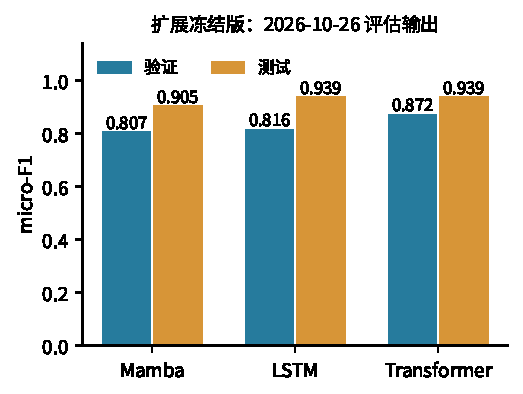
\includegraphics[width=\linewidth]{figures/expanded_results.pdf}
\caption{扩展冻结版本的验证／测试micro-F1。不同骨干处于同一记录阶段；未提供重复运行方差，故不绘制误差条。}
\label{fig:expanded}
\end{figure}

上述成绩支持系统在扩展数据阶段已经达到约0.94的测试F1。LSTM与Transformer的聚合P/R/F1相同，并不意味着它们对每个窗口的预测完全相同；需要逐单元输出才能比较错误分布。Mamba在该阶段的测试F1低3.4个百分点，而RSI的搜索空间包含骨干选择，因此应以最终胜者的实际配置描述交付模型，不能预先假定冠军一定是Mamba。

\subsection{最终全量结果的绑定}
\textbf{项目方确认的最终全量结果约为0.93，且经过多轮RSI优化。}这项结果应作为最终技术报告的核心成果，而非以初始五段实验替代。现阶段已经确认存在后续全量构建、132维特征、\code{rsi\_final}系列与LSTM模型demo；但最终0.93的完整指标键、精确值、数据索引SHA、冠军run与独立测试文件尚未由本次会话直接读取。

因此，本文将0.93保留为项目方最终结果，并将表\ref{tab:results}标为已经回收证据的扩展阶段结果。最终定稿应把冠军的指标行、精确测试样本数和配置补入主表，并用其同版本P/R/F1、每层指标和支持数更新分析。该步骤是来源绑定，不是要求重跑已完成的工作。

\subsection{不同版本之间的比较原则}
图\ref{fig:history}展示系统开发中的分阶段成绩。随着自动复核、数据扩充和训练配置变化，三个骨干的历史test F1均发生变化。由于测试采集、标注分布和输入条件并不固定，不能把柱值差分解释为RSI的纯粹因果增益。RSI收益应比较同一冻结数据、同一特征和同一评估口径下的初始配置与冠军。

全正预测的参照值依赖当前已知正负单元数，$F_1^{all+}=2P/(2P+N)$。初始五段子集的参照只适用于该子集，不能拿来与扩展版或最终全量0.93比较。正式报告应从最终benchmark重新读取TP/FP/FN及标签支持数，再计算同口径参照。

\begin{figure*}[t]
\centering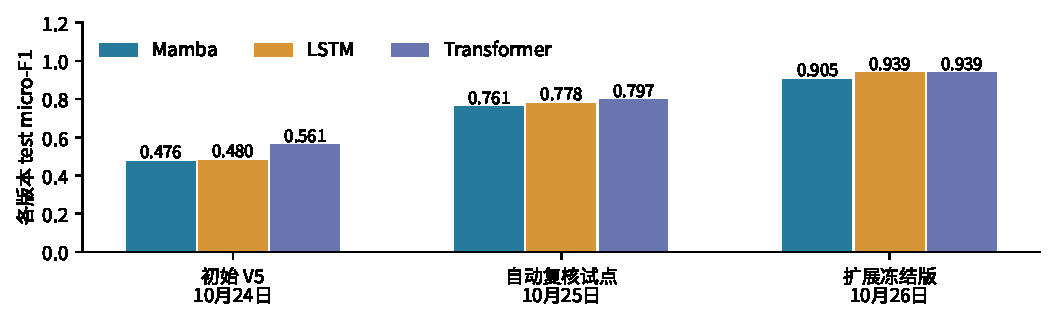
\includegraphics[width=\textwidth]{figures/version_history.pdf}
\caption{历史版本结果概览。每组柱对应各版本自身测试集，数据规模与监督发生变化，仅呈现项目演进，不作为固定测试集上的提升曲线，也不将最终0.93强行接到某个历史模型上。}
\label{fig:history}
\end{figure*}

\section{已完成的Demo与可视化}
\subsection{实际资产}
本地已存在六个项目演示视频，包括早期\code{b857b2a8\_demo}、放大版、位姿版、\code{demo\_v5}和\code{demo\_v6}。最新本地文件\code{demo\_v6.mp4}经读取确认长8秒、24帧、3fps、1500$\times$500像素，展示第一视角RGB、复核关系图和LSTM预测关系图三栏内容。该文件是已有演示，不是待从零制作的素材。

\begin{figure*}[t]
\centering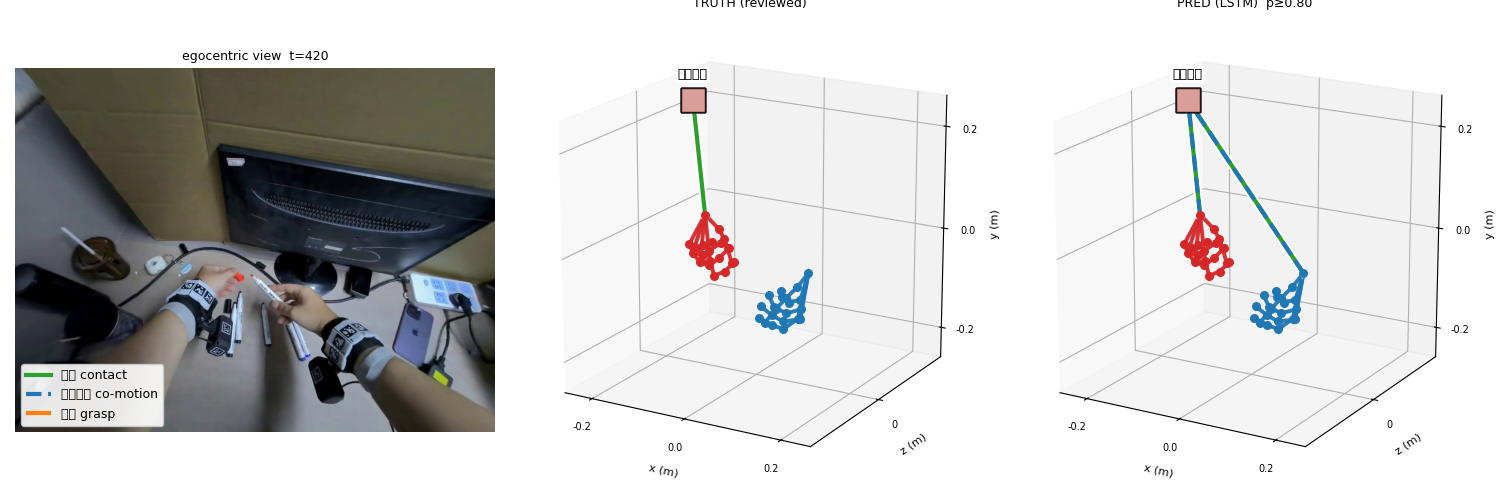
\includegraphics[width=\textwidth]{figures/demo_v6_actual.png}
\caption{现有demo v6真实预览帧。左为第一视角图像，中为已有复核关系，右为LSTM预测关系（画面阈值0.80）。手部骨架和物体位姿用于显示观测，模型预测的是交互边，不是未来三维姿态。原图保留，部分中文仍显示方框；正式导出应修复字体。原画面“TRUTH”不自动证明标签是独立人工金标准。}
\label{fig:demo}
\end{figure*}

迭代内容包括：修正类型编号到词表名称的映射；缩小三维展示范围并放大手部骨架；加入物体颜色、名称与姿态轴；改进几何名称关联；增加边类型图例与描边；以及选择连续帧以减少跳变。这些工作改善了可读性，但视频美观程度不替代模型评价。

\subsection{正式展示需要补齐的绑定}
已有demo使用LSTM及0.80显示阈值，而既有benchmark通常按0.5统计。展示阈值与评估阈值必须区分。正式视频应绑定最终RSI冠军checkpoint与数据版本，在同一历史窗口上输出概率，再于目标时刻揭示复核标签。显示的骨架属于观测值，应在图例中明确标注，避免观众误以为模型预测未来手部轨迹。

无位姿对象在旧版演示中可能回退为示意方块；正式素材建议显示“位姿缺失”，或者使用显式二维插图，避免把人为深度当作测量结果。模型预测、复核正负关系和未知区域也应使用不同的图例，不将未标注区域标成正确预测。

建议将现有短片作为90--120秒主片的中段：先介绍问题和系统，再展示冠军的连续预测与未来核验，随后给一个误报／漏报案例和一个未知片段，最后展示最终结果及同版本基线。分镜和具体文件清单见配套素材文档。

\section{复现与分析要求}
最终报告需统一四项版本绑定：数据索引与准入文件、特征版本、模型配置／checkpoint、评估器和指标口径。最终全量数据规模应从绑定索引统计，不将资源池、参与处理的采集数和产生有效监督的采集数混为同一数量。

132维增强的上游物体几何包含离线候选，因此在对外说明时应区分条件化预测与严格在线预测。若需要论证全自动实时使用，应单独评价感知误差、身份切换、别名匹配失败及端到端延迟；现有三栏回放不等于实时传感器系统。该边界不改变已完成的交互预测实验，而是明确其使用条件。

对于优化归因，应保留同版本初始配置、冠军配置和每次晋升的验证分数，再独立报告测试结果。最终轮数、成功候选数和数据扩充效果不能根据默认参数或目录名称推断。已有失败候选也应保留，避免搜索账本只剩最终成功项。

\section{结论}
本项目已形成从第一视角数据、视觉复核、手物特征到有向交互图预测的完整技术链，并在数据扩充、132维位姿增强与多系列RSI中持续优化。项目方报告最终全量结果约0.93；已恢复的扩展阶段原始评估记录显示test micro-F1达到0.939。系统还完成了多版三栏关系图demo。后续定稿重点是将最终冠军、全量索引和RSI谱系绑定到主结果表，并用同一模型生成正式展示素材。

{\small\bibliographystyle{ieeenat_fullname}\bibliography{references}}
\clearpage\appendix\balance
\section{本稿证据来源}
本稿直接检查了本地图模型、加载器、132维位姿模块、RSI脚本和自动复核实现；从历史会话恢复了原始工具返回的10月24--28日评估与规模摘要，以及11月4日后续训练记录。工具摘录保存在\code{evidence/later\_run\_outputs.json}，带原始时间戳；v4规模总结另存\code{stage\_summary\_excerpt.json}，明确其为历史总结而非原始索引。摘录不包含连接凭据或整个会话。

最终全量0.93来自本轮项目方明确说明。10月26日0.939来自已保存的评估输出；两者数值接近，但不能仅凭接近就认定是同一个checkpoint或同一数据版本。当前稿件因此标为“全流程结果对齐稿”。旧五段稿已归档为撤回版本，不再作为正式实验结论。

\section{最终同步入口}
优先读取数据盘\code{runs/rsi\_final}、\code{runs/rsi\_auto}与\code{runs/graph\_v5\_auto}；其中包括历史\code{lstm\_final}等模型目录及\code{demo\_videos}。需提取\code{history.jsonl}、\code{REPORT.md}、\code{genome.yaml}、成功候选的\code{score.json}、\code{config\_resolved.json}和最终\code{test\_benchmark.json}。候选目录必须与最终获选run对应。

数据端记录了\code{egodemo\_auto\_review\_20261025}与\code{egodemo\_auto\_review\_fasttrain}两条根目录。读取实际run中的数据路径后，再绑定对应索引、特征版本、划分与监督覆盖；不要仅按“final”或目录日期选择数据。位姿源为\code{egodemo\_refine\_300\_group6d\_20261025}系列，需与实际配置核对。

\section{正式图表清单}
建议正文保留系统结构、数据与版本演进、同版本主结果、RSI机制和真实demo五类图。补充材料增加RSI逐轮成绩／晋升曲线、最终四层交互指标与支持数、失败及未知案例、最终冠军配置。已有短片与截图可直接作为素材基础；重新渲染主要解决冠军绑定、时间边界、阈值说明、中文字体和缺失位姿显示。
\end{document}
